\documentclass[t,usenames,dvipsnames]{beamer}
\usetheme{Copenhagen}
\setbeamertemplate{headline}{} % remove toc from headers
\beamertemplatenavigationsymbolsempty

\usepackage{amsmath, tikz, xcolor, array, graphicx, pgf, pgfplots}
\pgfplotsset{compat=newest}
\usetikzlibrary{arrows.meta}
\usepgfplotslibrary{polar}
\everymath{\displaystyle}

\title{Graphs of Polar Equations}
\author{}
\date{}

\AtBeginSection[]
{
  \begin{frame}
    \frametitle{Objectives}
    \tableofcontents[currentsection]
  \end{frame}
}

\begin{document}

\begin{frame}
    \titlepage
\end{frame}

\section{Graph polar equations}

\begin{frame}{Example 1}
Graph each and comment on the graph.    \newline\\
(a) \quad $r = 4$   \pause \\[15pt]

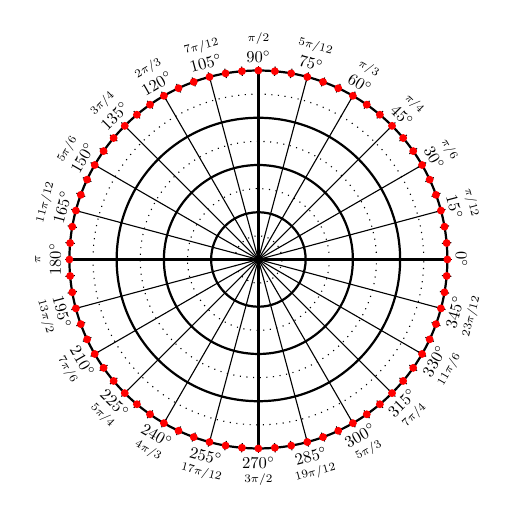
\begin{tikzpicture}[scale = 0.4, every node/.style={scale=0.6}]
    % Origin Point
    \coordinate (O) (0,0);
    % Circles
    \foreach \r in {1.5,3,...,6}
    {
        \draw[thick] (O) circle (\r cm);
    }
    
    % \foreach \r in {1.5,3,...7.5}
    % {
    %     \node at (\r, 0) [anchor=north] {\r/};
    % }
    
    \foreach \r in {0.75, 2.25,...,5.25}
    {
        \draw[dotted] (O) circle (\r cm);
    }
    
    % \node at (1.5, 0) [anchor = north west] {1};
    % \node at (3, 0) [anchor = north west] {2};
    % \node at (4.5, 0) [anchor = north west] {3};
    % \node at (6, 0) [anchor = north west] {4};
    % \node at (7.5,0) [anchor = north west] {5};
    % \foreach \r in {1.5,3,...,9}
    % {
    %     \node at (\r, 0) {\r/1.5};
    % }
    % Radial Lines
    \foreach \l in {0,15,...,360}
    {
        \draw (O) -- ++(\l:6cm);
    }
    % Thicker Radial Lines at 90 degree increments
    \foreach \l in {0,90,...,360}
    {
        \draw[very thick] (O) -- ++(\l:6cm);
    }
    % Minor Tick marks on outer circle
    \foreach \t in {0,5,...,360}
    {
        \draw (O) ++ (\t:5.85cm) -- ++(\t:0.3cm);
    }
    % Now for the fun part, the text
    % Degrees
    \node[draw=none, rotate= -90 ] at ( 0 :6.45cm) {$ 0 ^\circ$};
    \node[draw=none, rotate= -75 ] at ( 15 :6.45cm) {$ 15 ^\circ$};
    \node[draw=none, rotate= -60 ] at ( 30 :6.45cm) {$ 30 ^\circ$};
    \node[draw=none, rotate= -45 ] at ( 45 :6.45cm) {$ 45 ^\circ$};
    \node[draw=none, rotate= -30 ] at ( 60 :6.45cm) {$ 60 ^\circ$};
    \node[draw=none, rotate= -15 ] at ( 75 :6.45cm) {$ 75 ^\circ$};
    \node[draw=none, rotate= 0 ] at ( 90 :6.45cm) {$ 90 ^\circ$};
    \node[draw=none, rotate= 15 ] at ( 105 :6.45cm) {$ 105 ^\circ$};
    \node[draw=none, rotate= 30 ] at ( 120 :6.45cm) {$ 120 ^\circ$};
    \node[draw=none, rotate= 45 ] at ( 135 :6.45cm) {$ 135 ^\circ$};
    \node[draw=none, rotate= 60 ] at ( 150 :6.45cm) {$ 150 ^\circ$};
    \node[draw=none, rotate= 75 ] at ( 165 :6.45cm) {$ 165 ^\circ$};
    \node[draw=none, rotate= 90 ] at ( 180 :6.45cm) {$ 180 ^\circ$};
    \node[draw=none, rotate= 285 ] at ( 195 :6.45cm) {$ 195 ^\circ$};
    \node[draw=none, rotate= 300 ] at ( 210 :6.45cm) {$ 210 ^\circ$};
    \node[draw=none, rotate= 315 ] at ( 225 :6.45cm) {$ 225 ^\circ$};
    \node[draw=none, rotate= 330 ] at ( 240 :6.45cm) {$ 240 ^\circ$};
    \node[draw=none, rotate= 345 ] at ( 255 :6.45cm) {$ 255 ^\circ$};
    \node[draw=none, rotate= 360 ] at ( 270 :6.45cm) {$ 270 ^\circ$};
    \node[draw=none, rotate= 375 ] at ( 285 :6.45cm) {$ 285 ^\circ$};
    \node[draw=none, rotate= 390 ] at ( 300 :6.45cm) {$ 300 ^\circ$};
    \node[draw=none, rotate= 405 ] at ( 315 :6.45cm) {$ 315 ^\circ$};
    \node[draw=none, rotate= 420 ] at ( 330 :6.45cm) {$ 330 ^\circ$};
    \node[draw=none, rotate= 435 ] at ( 345 :6.45cm) {$ 345 ^\circ$};
    % Radians

    \node[draw=none, rotate= -90 ] at ( 0 :7cm) {$  $};
    \node[draw=none, rotate= -75 ] at ( 15 :7cm) {\scriptsize$ \pi/12 $};
    \node[draw=none, rotate= -60 ] at ( 30 :7cm) {\scriptsize$ \pi/6 $};
    \node[draw=none, rotate= -45 ] at ( 45 :7cm) {\scriptsize$ \pi/4 $};
    \node[draw=none, rotate= -30 ] at ( 60 :7cm) {\scriptsize$ \pi/3 $};
    \node[draw=none, rotate= -15 ] at ( 75 :7cm) {\scriptsize$ 5\pi/12 $};
    \node[draw=none, rotate= 0 ] at ( 90 :7cm) {\scriptsize$ \pi/2 $};
    \node[draw=none, rotate= 15 ] at ( 105 :7cm) {\scriptsize$ 7\pi/12 $};
    \node[draw=none, rotate= 30 ] at ( 120 :7cm) {\scriptsize$ 2\pi/3 $};
    \node[draw=none, rotate= 45 ] at ( 135 :7cm) {\scriptsize$ 3\pi/4 $};
    \node[draw=none, rotate= 60 ] at ( 150 :7cm) {\scriptsize$ 5\pi/6 $};
    \node[draw=none, rotate= 75 ] at ( 165 :7cm) {\scriptsize$ 11\pi/12 $};
    \node[draw=none, rotate= 90 ] at ( 180 :7cm) {\scriptsize$ \pi $};
    \node[draw=none, rotate= 285 ] at ( 195 :7cm) {\scriptsize$ 13\pi/2 $};
    \node[draw=none, rotate= 300 ] at ( 210 :7cm) {\scriptsize$ 7\pi/6 $};
    \node[draw=none, rotate= 315 ] at ( 225 :7cm) {\scriptsize$ 5\pi/4 $};
    \node[draw=none, rotate= 330 ] at ( 240 :7cm) {\scriptsize$ 4\pi/3 $};
    \node[draw=none, rotate= 345 ] at ( 255 :7cm) {\scriptsize$ 17\pi/12 $};
    \node[draw=none, rotate= 360 ] at ( 270 :7cm) {\scriptsize$ 3\pi/2 $};
    \node[draw=none, rotate= 375 ] at ( 285 :7cm) {\scriptsize$ 19\pi/12 $};
    \node[draw=none, rotate= 390 ] at ( 300 :7cm) {\scriptsize$ 5\pi/3 $};
    \node[draw=none, rotate= 405 ] at ( 315 :7cm) {\scriptsize$ 7\pi/4 $};
    \node[draw=none, rotate= 420 ] at ( 330 :7cm) {\scriptsize$ 11\pi/6 $};
    \node[draw=none, rotate= 435 ] at ( 345 :7cm) {\scriptsize$ 23\pi/12 $};
    
    \foreach \i in {0,5,...,355}
    \draw [color=red, fill=red] (\i:6cm) circle [radius=3pt];
\end{tikzpicture}
\end{frame}

\begin{frame}{Example 1}
(b) \quad $r = -3\sqrt{2}$  \\[15pt] \pause
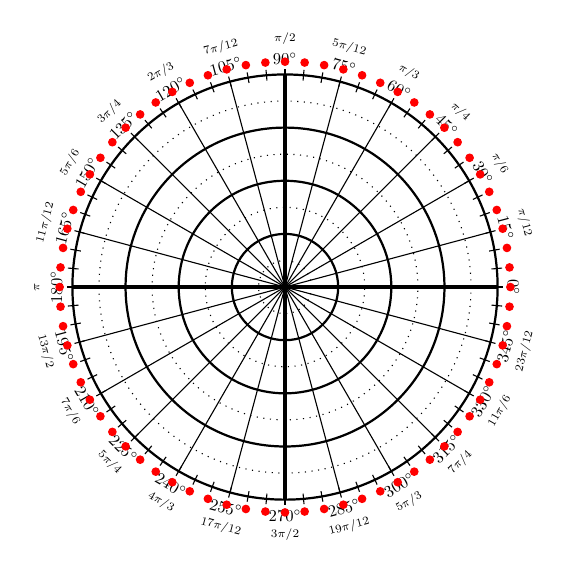
\begin{tikzpicture}[scale = 0.45, every node/.style={scale=0.6}]
    % Origin Point
    \coordinate (O) (0,0);
    % Circles
    \foreach \r in {1.5,3,...,6}
    {
        \draw[thick] (O) circle (\r cm);
    }
    
    % \foreach \r in {1.5,3,...7.5}
    % {
    %     \node at (\r, 0) [anchor=north] {\r/};
    % }
    
    \foreach \r in {0.75, 2.25,...,5.25}
    {
        \draw[dotted] (O) circle (\r cm);
    }
    
    % \node at (1.5, 0) [anchor = north west] {1};
    % \node at (3, 0) [anchor = north west] {2};
    % \node at (4.5, 0) [anchor = north west] {3};
    % \node at (6, 0) [anchor = north west] {4};
    % \node at (7.5,0) [anchor = north west] {5};
    % \foreach \r in {1.5,3,...,9}
    % {
    %     \node at (\r, 0) {\r/1.5};
    % }
    % Radial Lines
    \foreach \l in {0,15,...,360}
    {
        \draw (O) -- ++(\l:6cm);
    }
    % Thicker Radial Lines at 90 degree increments
    \foreach \l in {0,90,...,360}
    {
        \draw[very thick] (O) -- ++(\l:6cm);
    }
    % Minor Tick marks on outer circle
    \foreach \t in {0,5,...,360}
    {
        \draw (O) ++ (\t:5.85cm) -- ++(\t:0.3cm);
    }
    % Now for the fun part, the text
    % Degrees
    \node[draw=none, rotate= -90 ] at ( 0 :6.45cm) {$ 0 ^\circ$};
    \node[draw=none, rotate= -75 ] at ( 15 :6.45cm) {$ 15 ^\circ$};
    \node[draw=none, rotate= -60 ] at ( 30 :6.45cm) {$ 30 ^\circ$};
    \node[draw=none, rotate= -45 ] at ( 45 :6.45cm) {$ 45 ^\circ$};
    \node[draw=none, rotate= -30 ] at ( 60 :6.45cm) {$ 60 ^\circ$};
    \node[draw=none, rotate= -15 ] at ( 75 :6.45cm) {$ 75 ^\circ$};
    \node[draw=none, rotate= 0 ] at ( 90 :6.45cm) {$ 90 ^\circ$};
    \node[draw=none, rotate= 15 ] at ( 105 :6.45cm) {$ 105 ^\circ$};
    \node[draw=none, rotate= 30 ] at ( 120 :6.45cm) {$ 120 ^\circ$};
    \node[draw=none, rotate= 45 ] at ( 135 :6.45cm) {$ 135 ^\circ$};
    \node[draw=none, rotate= 60 ] at ( 150 :6.45cm) {$ 150 ^\circ$};
    \node[draw=none, rotate= 75 ] at ( 165 :6.45cm) {$ 165 ^\circ$};
    \node[draw=none, rotate= 90 ] at ( 180 :6.45cm) {$ 180 ^\circ$};
    \node[draw=none, rotate= 285 ] at ( 195 :6.45cm) {$ 195 ^\circ$};
    \node[draw=none, rotate= 300 ] at ( 210 :6.45cm) {$ 210 ^\circ$};
    \node[draw=none, rotate= 315 ] at ( 225 :6.45cm) {$ 225 ^\circ$};
    \node[draw=none, rotate= 330 ] at ( 240 :6.45cm) {$ 240 ^\circ$};
    \node[draw=none, rotate= 345 ] at ( 255 :6.45cm) {$ 255 ^\circ$};
    \node[draw=none, rotate= 360 ] at ( 270 :6.45cm) {$ 270 ^\circ$};
    \node[draw=none, rotate= 375 ] at ( 285 :6.45cm) {$ 285 ^\circ$};
    \node[draw=none, rotate= 390 ] at ( 300 :6.45cm) {$ 300 ^\circ$};
    \node[draw=none, rotate= 405 ] at ( 315 :6.45cm) {$ 315 ^\circ$};
    \node[draw=none, rotate= 420 ] at ( 330 :6.45cm) {$ 330 ^\circ$};
    \node[draw=none, rotate= 435 ] at ( 345 :6.45cm) {$ 345 ^\circ$};
    % Radians

    \node[draw=none, rotate= -90 ] at ( 0 :7cm) {$  $};
    \node[draw=none, rotate= -75 ] at ( 15 :7cm) {\scriptsize$ \pi/12 $};
    \node[draw=none, rotate= -60 ] at ( 30 :7cm) {\scriptsize$ \pi/6 $};
    \node[draw=none, rotate= -45 ] at ( 45 :7cm) {\scriptsize$ \pi/4 $};
    \node[draw=none, rotate= -30 ] at ( 60 :7cm) {\scriptsize$ \pi/3 $};
    \node[draw=none, rotate= -15 ] at ( 75 :7cm) {\scriptsize$ 5\pi/12 $};
    \node[draw=none, rotate= 0 ] at ( 90 :7cm) {\scriptsize$ \pi/2 $};
    \node[draw=none, rotate= 15 ] at ( 105 :7cm) {\scriptsize$ 7\pi/12 $};
    \node[draw=none, rotate= 30 ] at ( 120 :7cm) {\scriptsize$ 2\pi/3 $};
    \node[draw=none, rotate= 45 ] at ( 135 :7cm) {\scriptsize$ 3\pi/4 $};
    \node[draw=none, rotate= 60 ] at ( 150 :7cm) {\scriptsize$ 5\pi/6 $};
    \node[draw=none, rotate= 75 ] at ( 165 :7cm) {\scriptsize$ 11\pi/12 $};
    \node[draw=none, rotate= 90 ] at ( 180 :7cm) {\scriptsize$ \pi $};
    \node[draw=none, rotate= 285 ] at ( 195 :7cm) {\scriptsize$ 13\pi/2 $};
    \node[draw=none, rotate= 300 ] at ( 210 :7cm) {\scriptsize$ 7\pi/6 $};
    \node[draw=none, rotate= 315 ] at ( 225 :7cm) {\scriptsize$ 5\pi/4 $};
    \node[draw=none, rotate= 330 ] at ( 240 :7cm) {\scriptsize$ 4\pi/3 $};
    \node[draw=none, rotate= 345 ] at ( 255 :7cm) {\scriptsize$ 17\pi/12 $};
    \node[draw=none, rotate= 360 ] at ( 270 :7cm) {\scriptsize$ 3\pi/2 $};
    \node[draw=none, rotate= 375 ] at ( 285 :7cm) {\scriptsize$ 19\pi/12 $};
    \node[draw=none, rotate= 390 ] at ( 300 :7cm) {\scriptsize$ 5\pi/3 $};
    \node[draw=none, rotate= 405 ] at ( 315 :7cm) {\scriptsize$ 7\pi/4 $};
    \node[draw=none, rotate= 420 ] at ( 330 :7cm) {\scriptsize$ 11\pi/6 $};
    \node[draw=none, rotate= 435 ] at ( 345 :7cm) {\scriptsize$ 23\pi/12 $};
    
    \foreach \i in {0,5,...,355}
    \draw [color=red, fill=red] (\i:6.36) circle [radius=3pt];
\end{tikzpicture}
\end{frame}

\begin{frame}{Example 1}
(c) \quad $\theta = \dfrac{5\pi}{4}$    \newline\\  \pause
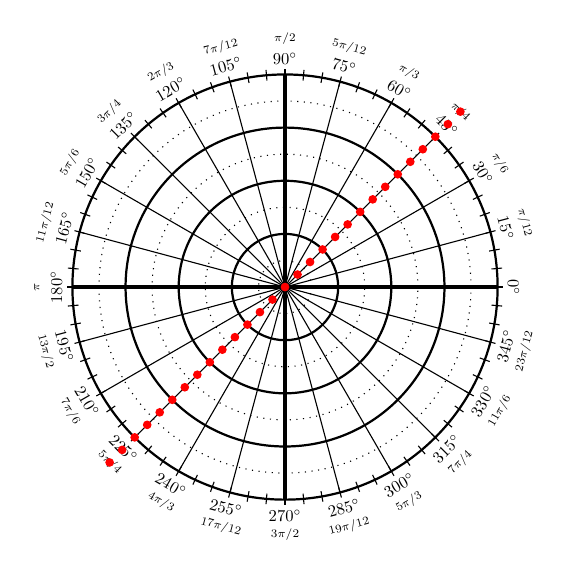
\begin{tikzpicture}[scale = 0.45, every node/.style={scale=0.6}]
    % Origin Point
    \coordinate (O) (0,0);
    % Circles
    \foreach \r in {1.5,3,...,6}
    {
        \draw[thick] (O) circle (\r cm);
    }
    
    % \foreach \r in {1.5,3,...7.5}
    % {
    %     \node at (\r, 0) [anchor=north] {\r/};
    % }
    
    \foreach \r in {0.75, 2.25,...,5.25}
    {
        \draw[dotted] (O) circle (\r cm);
    }
    
    % \node at (1.5, 0) [anchor = north west] {1};
    % \node at (3, 0) [anchor = north west] {2};
    % \node at (4.5, 0) [anchor = north west] {3};
    % \node at (6, 0) [anchor = north west] {4};
    % \node at (7.5,0) [anchor = north west] {5};
    % \foreach \r in {1.5,3,...,9}
    % {
    %     \node at (\r, 0) {\r/1.5};
    % }
    % Radial Lines
    \foreach \l in {0,15,...,360}
    {
        \draw (O) -- ++(\l:6cm);
    }
    % Thicker Radial Lines at 90 degree increments
    \foreach \l in {0,90,...,360}
    {
        \draw[very thick] (O) -- ++(\l:6cm);
    }
    % Minor Tick marks on outer circle
    \foreach \t in {0,5,...,360}
    {
        \draw (O) ++ (\t:5.85cm) -- ++(\t:0.3cm);
    }
    % Now for the fun part, the text
    % Degrees
    \node[draw=none, rotate= -90 ] at ( 0 :6.45cm) {$ 0 ^\circ$};
    \node[draw=none, rotate= -75 ] at ( 15 :6.45cm) {$ 15 ^\circ$};
    \node[draw=none, rotate= -60 ] at ( 30 :6.45cm) {$ 30 ^\circ$};
    \node[draw=none, rotate= -45 ] at ( 45 :6.45cm) {$ 45 ^\circ$};
    \node[draw=none, rotate= -30 ] at ( 60 :6.45cm) {$ 60 ^\circ$};
    \node[draw=none, rotate= -15 ] at ( 75 :6.45cm) {$ 75 ^\circ$};
    \node[draw=none, rotate= 0 ] at ( 90 :6.45cm) {$ 90 ^\circ$};
    \node[draw=none, rotate= 15 ] at ( 105 :6.45cm) {$ 105 ^\circ$};
    \node[draw=none, rotate= 30 ] at ( 120 :6.45cm) {$ 120 ^\circ$};
    \node[draw=none, rotate= 45 ] at ( 135 :6.45cm) {$ 135 ^\circ$};
    \node[draw=none, rotate= 60 ] at ( 150 :6.45cm) {$ 150 ^\circ$};
    \node[draw=none, rotate= 75 ] at ( 165 :6.45cm) {$ 165 ^\circ$};
    \node[draw=none, rotate= 90 ] at ( 180 :6.45cm) {$ 180 ^\circ$};
    \node[draw=none, rotate= 285 ] at ( 195 :6.45cm) {$ 195 ^\circ$};
    \node[draw=none, rotate= 300 ] at ( 210 :6.45cm) {$ 210 ^\circ$};
    \node[draw=none, rotate= 315 ] at ( 225 :6.45cm) {$ 225 ^\circ$};
    \node[draw=none, rotate= 330 ] at ( 240 :6.45cm) {$ 240 ^\circ$};
    \node[draw=none, rotate= 345 ] at ( 255 :6.45cm) {$ 255 ^\circ$};
    \node[draw=none, rotate= 360 ] at ( 270 :6.45cm) {$ 270 ^\circ$};
    \node[draw=none, rotate= 375 ] at ( 285 :6.45cm) {$ 285 ^\circ$};
    \node[draw=none, rotate= 390 ] at ( 300 :6.45cm) {$ 300 ^\circ$};
    \node[draw=none, rotate= 405 ] at ( 315 :6.45cm) {$ 315 ^\circ$};
    \node[draw=none, rotate= 420 ] at ( 330 :6.45cm) {$ 330 ^\circ$};
    \node[draw=none, rotate= 435 ] at ( 345 :6.45cm) {$ 345 ^\circ$};
    % Radians

    \node[draw=none, rotate= -90 ] at ( 0 :7cm) {$  $};
    \node[draw=none, rotate= -75 ] at ( 15 :7cm) {\scriptsize$ \pi/12 $};
    \node[draw=none, rotate= -60 ] at ( 30 :7cm) {\scriptsize$ \pi/6 $};
    \node[draw=none, rotate= -45 ] at ( 45 :7cm) {\scriptsize$ \pi/4 $};
    \node[draw=none, rotate= -30 ] at ( 60 :7cm) {\scriptsize$ \pi/3 $};
    \node[draw=none, rotate= -15 ] at ( 75 :7cm) {\scriptsize$ 5\pi/12 $};
    \node[draw=none, rotate= 0 ] at ( 90 :7cm) {\scriptsize$ \pi/2 $};
    \node[draw=none, rotate= 15 ] at ( 105 :7cm) {\scriptsize$ 7\pi/12 $};
    \node[draw=none, rotate= 30 ] at ( 120 :7cm) {\scriptsize$ 2\pi/3 $};
    \node[draw=none, rotate= 45 ] at ( 135 :7cm) {\scriptsize$ 3\pi/4 $};
    \node[draw=none, rotate= 60 ] at ( 150 :7cm) {\scriptsize$ 5\pi/6 $};
    \node[draw=none, rotate= 75 ] at ( 165 :7cm) {\scriptsize$ 11\pi/12 $};
    \node[draw=none, rotate= 90 ] at ( 180 :7cm) {\scriptsize$ \pi $};
    \node[draw=none, rotate= 285 ] at ( 195 :7cm) {\scriptsize$ 13\pi/2 $};
    \node[draw=none, rotate= 300 ] at ( 210 :7cm) {\scriptsize$ 7\pi/6 $};
    \node[draw=none, rotate= 315 ] at ( 225 :7cm) {\scriptsize$ 5\pi/4 $};
    \node[draw=none, rotate= 330 ] at ( 240 :7cm) {\scriptsize$ 4\pi/3 $};
    \node[draw=none, rotate= 345 ] at ( 255 :7cm) {\scriptsize$ 17\pi/12 $};
    \node[draw=none, rotate= 360 ] at ( 270 :7cm) {\scriptsize$ 3\pi/2 $};
    \node[draw=none, rotate= 375 ] at ( 285 :7cm) {\scriptsize$ 19\pi/12 $};
    \node[draw=none, rotate= 390 ] at ( 300 :7cm) {\scriptsize$ 5\pi/3 $};
    \node[draw=none, rotate= 405 ] at ( 315 :7cm) {\scriptsize$ 7\pi/4 $};
    \node[draw=none, rotate= 420 ] at ( 330 :7cm) {\scriptsize$ 11\pi/6 $};
    \node[draw=none, rotate= 435 ] at ( 345 :7cm) {\scriptsize$ 23\pi/12 $};
    
    \foreach \i in {-7,-6.5,...,7}
    \draw [color=red, fill=red] (225:\i) circle [radius=3pt];
\end{tikzpicture} 
\end{frame}

\begin{frame}{Example 1}
(d) \quad $\theta = -\dfrac{3\pi}{2}$    \newline\\  \pause
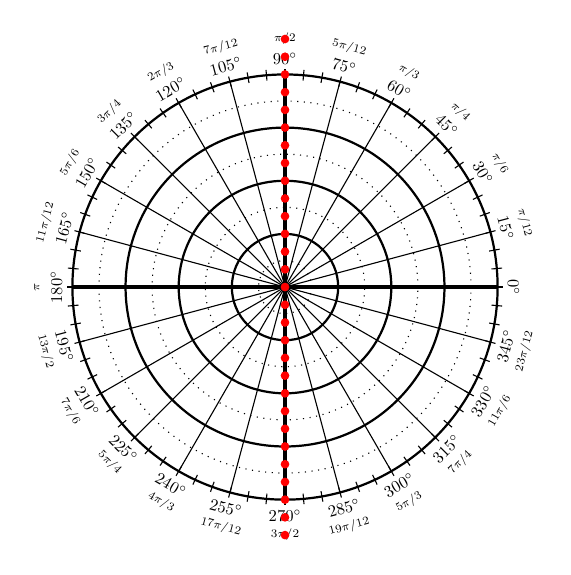
\begin{tikzpicture}[scale = 0.45, every node/.style={scale=0.6}]
    % Origin Point
    \coordinate (O) (0,0);
    % Circles
    \foreach \r in {1.5,3,...,6}
    {
        \draw[thick] (O) circle (\r cm);
    }
    
    % \foreach \r in {1.5,3,...7.5}
    % {
    %     \node at (\r, 0) [anchor=north] {\r/};
    % }
    
    \foreach \r in {0.75, 2.25,...,5.25}
    {
        \draw[dotted] (O) circle (\r cm);
    }
    
    % \node at (1.5, 0) [anchor = north west] {1};
    % \node at (3, 0) [anchor = north west] {2};
    % \node at (4.5, 0) [anchor = north west] {3};
    % \node at (6, 0) [anchor = north west] {4};
    % \node at (7.5,0) [anchor = north west] {5};
    % \foreach \r in {1.5,3,...,9}
    % {
    %     \node at (\r, 0) {\r/1.5};
    % }
    % Radial Lines
    \foreach \l in {0,15,...,360}
    {
        \draw (O) -- ++(\l:6cm);
    }
    % Thicker Radial Lines at 90 degree increments
    \foreach \l in {0,90,...,360}
    {
        \draw[very thick] (O) -- ++(\l:6cm);
    }
    % Minor Tick marks on outer circle
    \foreach \t in {0,5,...,360}
    {
        \draw (O) ++ (\t:5.85cm) -- ++(\t:0.3cm);
    }
    % Now for the fun part, the text
    % Degrees
    \node[draw=none, rotate= -90 ] at ( 0 :6.45cm) {$ 0 ^\circ$};
    \node[draw=none, rotate= -75 ] at ( 15 :6.45cm) {$ 15 ^\circ$};
    \node[draw=none, rotate= -60 ] at ( 30 :6.45cm) {$ 30 ^\circ$};
    \node[draw=none, rotate= -45 ] at ( 45 :6.45cm) {$ 45 ^\circ$};
    \node[draw=none, rotate= -30 ] at ( 60 :6.45cm) {$ 60 ^\circ$};
    \node[draw=none, rotate= -15 ] at ( 75 :6.45cm) {$ 75 ^\circ$};
    \node[draw=none, rotate= 0 ] at ( 90 :6.45cm) {$ 90 ^\circ$};
    \node[draw=none, rotate= 15 ] at ( 105 :6.45cm) {$ 105 ^\circ$};
    \node[draw=none, rotate= 30 ] at ( 120 :6.45cm) {$ 120 ^\circ$};
    \node[draw=none, rotate= 45 ] at ( 135 :6.45cm) {$ 135 ^\circ$};
    \node[draw=none, rotate= 60 ] at ( 150 :6.45cm) {$ 150 ^\circ$};
    \node[draw=none, rotate= 75 ] at ( 165 :6.45cm) {$ 165 ^\circ$};
    \node[draw=none, rotate= 90 ] at ( 180 :6.45cm) {$ 180 ^\circ$};
    \node[draw=none, rotate= 285 ] at ( 195 :6.45cm) {$ 195 ^\circ$};
    \node[draw=none, rotate= 300 ] at ( 210 :6.45cm) {$ 210 ^\circ$};
    \node[draw=none, rotate= 315 ] at ( 225 :6.45cm) {$ 225 ^\circ$};
    \node[draw=none, rotate= 330 ] at ( 240 :6.45cm) {$ 240 ^\circ$};
    \node[draw=none, rotate= 345 ] at ( 255 :6.45cm) {$ 255 ^\circ$};
    \node[draw=none, rotate= 360 ] at ( 270 :6.45cm) {$ 270 ^\circ$};
    \node[draw=none, rotate= 375 ] at ( 285 :6.45cm) {$ 285 ^\circ$};
    \node[draw=none, rotate= 390 ] at ( 300 :6.45cm) {$ 300 ^\circ$};
    \node[draw=none, rotate= 405 ] at ( 315 :6.45cm) {$ 315 ^\circ$};
    \node[draw=none, rotate= 420 ] at ( 330 :6.45cm) {$ 330 ^\circ$};
    \node[draw=none, rotate= 435 ] at ( 345 :6.45cm) {$ 345 ^\circ$};
    % Radians

    \node[draw=none, rotate= -90 ] at ( 0 :7cm) {$  $};
    \node[draw=none, rotate= -75 ] at ( 15 :7cm) {\scriptsize$ \pi/12 $};
    \node[draw=none, rotate= -60 ] at ( 30 :7cm) {\scriptsize$ \pi/6 $};
    \node[draw=none, rotate= -45 ] at ( 45 :7cm) {\scriptsize$ \pi/4 $};
    \node[draw=none, rotate= -30 ] at ( 60 :7cm) {\scriptsize$ \pi/3 $};
    \node[draw=none, rotate= -15 ] at ( 75 :7cm) {\scriptsize$ 5\pi/12 $};
    \node[draw=none, rotate= 0 ] at ( 90 :7cm) {\scriptsize$ \pi/2 $};
    \node[draw=none, rotate= 15 ] at ( 105 :7cm) {\scriptsize$ 7\pi/12 $};
    \node[draw=none, rotate= 30 ] at ( 120 :7cm) {\scriptsize$ 2\pi/3 $};
    \node[draw=none, rotate= 45 ] at ( 135 :7cm) {\scriptsize$ 3\pi/4 $};
    \node[draw=none, rotate= 60 ] at ( 150 :7cm) {\scriptsize$ 5\pi/6 $};
    \node[draw=none, rotate= 75 ] at ( 165 :7cm) {\scriptsize$ 11\pi/12 $};
    \node[draw=none, rotate= 90 ] at ( 180 :7cm) {\scriptsize$ \pi $};
    \node[draw=none, rotate= 285 ] at ( 195 :7cm) {\scriptsize$ 13\pi/2 $};
    \node[draw=none, rotate= 300 ] at ( 210 :7cm) {\scriptsize$ 7\pi/6 $};
    \node[draw=none, rotate= 315 ] at ( 225 :7cm) {\scriptsize$ 5\pi/4 $};
    \node[draw=none, rotate= 330 ] at ( 240 :7cm) {\scriptsize$ 4\pi/3 $};
    \node[draw=none, rotate= 345 ] at ( 255 :7cm) {\scriptsize$ 17\pi/12 $};
    \node[draw=none, rotate= 360 ] at ( 270 :7cm) {\scriptsize$ 3\pi/2 $};
    \node[draw=none, rotate= 375 ] at ( 285 :7cm) {\scriptsize$ 19\pi/12 $};
    \node[draw=none, rotate= 390 ] at ( 300 :7cm) {\scriptsize$ 5\pi/3 $};
    \node[draw=none, rotate= 405 ] at ( 315 :7cm) {\scriptsize$ 7\pi/4 $};
    \node[draw=none, rotate= 420 ] at ( 330 :7cm) {\scriptsize$ 11\pi/6 $};
    \node[draw=none, rotate= 435 ] at ( 345 :7cm) {\scriptsize$ 23\pi/12 $};
    
    \foreach \i in {-7,-6.5,...,7}
    \draw [color=red, fill=red] (90:\i) circle [radius=3pt];
\end{tikzpicture} 
\end{frame}

\begin{frame}{$r = \#$ and $\theta = \#$}
    \begin{itemize}
        \item $r = \#$ is a circle with center at origin and radius = the absolute value of that number.  \newline\\  \pause
        \item $\theta = \#$ is a line through origin with slope = tangent of that number.
    \end{itemize}
\end{frame}

\begin{frame}{Example 2}
Graph each of the following and comment on the graph.   \newline\\
(a) \quad $r = 6\cos\theta$ \newline\\  \pause
\begin{itemize}
    \item Circle    \newline\\  \pause
    \item Center at $(3,0)$ \newline\\  \pause
    \item Diameter = 6
\end{itemize}
\end{frame}

\begin{frame}{Example 2}
(b) \quad $r = 4 - 2\sin\theta$ \newline\\  \pause
\begin{itemize}
    \item Lima\c{c}on  \newline\\  \pause
    \item $x$-intercepts at $(\pm 4,0)$ \newline\\  \pause
    \item $y$-intercepts at $(0,2)$ and $(0,-6)$
\end{itemize}
\end{frame}

\begin{frame}{Example 2}
(c) \quad $r = 2 + 4\cos\theta$ \newline\\  \pause
\begin{itemize}
    \item Lima\c{c}on \newline\\ \pause
    \item $x$-intercepts at $(0,0)$, $(2,0)$ and $(6,0)$ \newline\\ \pause
    \item $y$-intercepts at $(0, \pm 2)$    \newline\\ \pause
    \item Inner-loop diameter = 2   \newline\\  \pause
    \item Outer-loop diameter = 6
\end{itemize}
\end{frame}

\begin{frame}{Example 2}
(d) \quad $r = 5\sin(2\theta)$ \newline\\ \pause
\begin{itemize}
    \item Rose \newline\\ \pause
    \item Radius = 5 \newline\\ \pause
    \item 4 petals \newline\\  \pause
    \item No petals on an axis
\end{itemize}
\end{frame}

\begin{frame}{Example 2}
(e) \quad $r^2 = 16\cos(2\theta)$ \newline\\ \pause 
\[r = \pm 4\sqrt{\cos(2\theta)}\]   \pause
\begin{itemize}
    \item Lemniscate \newline\\ \pause
    \item $x$-intercepts at $(0,0)$ and $(\pm 4,0)$ \newline\\  \pause
    \item $y$-intercept at $(0,0)$
\end{itemize}
\end{frame}

\section{Find the intersection of polar equations}

\begin{frame}{Finding intersections of polar equations}
    Solving these will use elements of solving trigonometric equations. \newline\\    \pause
    Use graphing capabilities to check for intersection at the pole (origin).
\end{frame}

\begin{frame}{Example 3}
Find all exact points of intersection for each pair of equations.   \newline\\
(a) \quad $r = 2\sin\theta$ and $r = 2-2\sin\theta$ \newline\\  \pause
Graphs intersect at pole.
\begin{align*}
    \onslide<3->{2\sin \theta &= 2 - 2\sin\theta} \\[6pt]
    \onslide<4->{4\sin\theta &= 2} \\[6pt]
    \onslide<5->{\sin\theta &= \frac{1}{2}} \\[6pt]
    \onslide<6->{\theta &= \frac{\pi}{6}, \frac{5\pi}{6}}
\end{align*}
\end{frame}

\begin{frame}{Example 3 \quad $r = 2\sin\theta$ and $r = 2-2\sin\theta$}
\[\theta = \frac{\pi}{6}, \frac{5\pi}{6}  \]
\begin{align*}
    \onslide<2->{r &= 2\sin\left(\frac{\pi}{6}\right) & r &= 2\sin\left(\frac{5\pi}{6}\right)} \\[8pt]
    \onslide<3->{r &= 1 & r &= 1}
\end{align*}
\onslide<4->{\[\text{pole}, \quad \left(1,\frac{\pi}{6}\right), \quad \left(1, \frac{5\pi}{6}\right)\]}
\end{frame}


\begin{frame}{Example 3}
(b) \quad $r = 2$ and $r = 3\cos\theta$
\begin{align*}
    \onslide<2->{3\cos\theta &= 2}  \\[6pt]
    \onslide<3->{\cos\theta &= \frac{2}{3}} \\[6pt]
    \onslide<4->{\theta &= \arccos\left(\frac{2}{3}\right)} 
    \onslide<5->{\approx 48.2^\circ} \\[6pt]
\end{align*}
\begin{align*}
    \onslide<6->{&\left(2, 48.2^\circ\right) & \left(2, 311.8^\circ\right)} \\[6pt]
    \onslide<7->{&\left(2, \arccos\left(\frac{2}{3}\right)\right) & \left(2, 2\pi - \arccos\left(\frac{2}{3}\right)\right)}
\end{align*}
\end{frame}

\begin{frame}{Example 3}
(c) \quad $r = 3$ and $r = 6\cos(2\theta)$
\begin{align*}
    \onslide<2->{6\cos(2\theta) &= 3} \\[6pt]
    \onslide<3->{\cos(2\theta) &= \frac{1}{2}}
\end{align*}
\begin{align*}
    \onslide<4->{2\theta &= 60^\circ + 360n & 2\theta &= 300^\circ + 360n} \\[6pt]
    \onslide<5->{\theta &= 30^\circ + 180n & \theta &= 150^\circ + 180n} \\[6pt]
    \onslide<6->{\theta &= 30^\circ, \, 210^\circ & \theta &= 150^\circ, \, 330^\circ}
\end{align*}
\onslide<7->{\[\left(3, 30^\circ\right), \quad \left(3, 150^\circ\right), \quad \left(3, 210^\circ\right), \quad \left(3, 330^\circ\right)\]}
\end{frame}

\begin{frame}{Example 3}
(c) \quad     $r = 3$ and $r = 6\cos(2\theta)$
\begin{align*}
    \onslide<2->{6\cos(2\theta) &= -3} \\[6pt]
    \onslide<3->{\cos(2\theta) &= -\frac{1}{2}} 
\end{align*}
\begin{align*}
    \onslide<4->{2\theta &= 120^\circ + 360n & 2\theta &= 240^\circ + 360n} \\[6pt]
    \onslide<5->{\theta &= 60^\circ + 180n & \theta &= 120^\circ + 180n} \\[6pt]
    \onslide<6->{\theta &= 60^\circ, \, 240^\circ & \theta &= 120^\circ, \, 300^\circ}
\end{align*}
\onslide<7->{\[\left(-3, 60^\circ\right), \quad \left(-3, 120^\circ\right), \quad \left(-3, 240^\circ\right), \quad \left(-3, 300^\circ\right)\]}
\end{frame}

\begin{frame}{Example 3}
(c) \quad     $r = 3$ and $r = 6\cos(2\theta)$
\begin{align*}
    &\left(3, 30^\circ\right), \quad \left(3, 150^\circ\right), \quad \left(3, 210^\circ\right), \quad \left(3, 330^\circ\right) \\[8pt]
    &{\color{red}\left(3, \frac{\pi}{6}\right), \quad \left(3, \frac{5\pi}{6}\right), \quad \left(3, \frac{7\pi}{6}\right), \quad \left(3, \frac{11\pi}{6}\right)}   \\[12pt]
    &\left(-3, 60^\circ\right), \quad \left(-3, 120^\circ\right), \quad \left(-3, 240^\circ\right), \quad \left(-3, 300^\circ\right)    \\[8pt]
    &{\color{red}\left(-3, \frac{\pi}{3}\right), \quad \left(-3, \frac{2\pi}{3}\right), \quad \left(-3, \frac{4\pi}{3}\right), \quad \left(-3, \frac{5\pi}{3}\right)}   
\end{align*}
\end{frame}




\end{document}
